\section{Related Work}

This section reviews prior work relevant to the design
and implementation of spatial acceleration structures,
focusing on volume hierarchies, selection algorithms,
and practical open-source libraries. We highlight where
\texttt{tf::tree} aligns with or diverges from these approaches.

\subsection{Spatial Hierarchies and Partitioning}

Bounding volume hierarchies (BVHs) \cite{bvh-survey} are a foundational technique
in spatial queries, collision detection, and ray tracing.
Variants such as AABB trees\cite{van1997efficient},
kD-trees\cite{bentley1975multidimensional},
BIHs\cite{wachter2006instant}, and R-Trees\cite{r-tree} differ in their
partitioning schemes and traversal heuristics, but all aim to
minimize overlap and traversal cost. Common BVH construction
strategies include top-down recursive partitioning,
bottom-up agglomeration, and hybrid methods.

Many BVH builders use heuristics like the Surface Area Heuristic
(SAH)\cite{macdonald1990heuristics}
to guide node splitting. While SAH produces high-quality
trees, its exact evaluation is computationally expensive,
and n-ary balanced trees offer a trade-off between construction
and traversal efficiency.

SAH is primarily optimized for ray tracing, where the
goal is to minimize the expected cost of directional
queries such as ray intersections. This can lead to
deep, unbalanced trees that favor sparse, single-ray
workloads. In contrast, the queries we target—such as
collisions, intersections, and proximity searches—are
dense, symmetric, and involve pairwise interactions
between primitives. These tasks benefit from shallower,
balanced n-ary hierarchies that distribute work more uniformly
and reduce traversal depth. We therefore focus on
building balanced trees rather than optimizing for
expected ray traversal cost.

\subsubsection{Binning Approaches}

Binning is widely used to accelerate SAH evaluation by discretizing
the spatial domain and approximating split costs across bins~\cite{wald2007fast}.
This reduces the complexity of finding optimal partitions and enables
SAH-based builders to achieve the optimal $\mathcal{O}(n \log n)$
construction complexity~\cite{kdtreeologn}. However, it introduces
sensitivity to bin count, spatial distribution, and workload assumptions.

In contrast, \texttt{tf::tree} targets a broader class of spatial queries
that benefit from shallow, balanced hierarchies. It avoids binning entirely
by using in-place partitioning via state-of-the-art selection algorithms,
which ensures
$\mathcal{O}(n \log n)$ average-case construction. This approach simplifies
implementation, improves cache behavior, and supports query workloads
like intersection and proximity, where n-ary balanced depth often outperforms
heuristic-driven binary splits.

\subsection{Selection Algorithms}

While partitioning is central to spatial data structures,
much of the literature has focused on full sorting~\cite{str-tree}
or binning heuristics optimized for directional queries.
In contrast, the role of linear-time selection algorithms for computing
balanced splits has received comparatively little attention—despite
their potential benefits for general-purpose acceleration structures.

A long line of research has developed efficient algorithms for
finding order statistics in linear or near-linear time, beginning
with the Median of Medians algorithm~\cite{mom}, followed by
improvements such as Floyd--Rivest selection~\cite{floyd1975expected}
and more recent high-performance variants like PDQSelect~\cite{pdqSort},
and Median of Ninthers (Alexandrescu’s algorithm)~\cite{alexandrescu-sorting}.

\texttt{tf::tree} builds on this foundation by exposing the partitioning
strategy as a template parameter, enabling interchangeable use of these
algorithms during construction. In our experiments,
\texttt{std::nth\_element} consistently offers the best trade-off between
speed, cache behavior, and determinism—making it a practical choice
for in-place spatial partitioning in general workloads.

\subsection{Nearness Queries and Traversal Strategies}

Proximity queries, such as nearest-neighbor and
$k$-nearest-neighbor searches, are fundamental operations in spatial data
structures. R-trees~\cite{knn0} commonly employ best-first traversal
strategies using priority queues to order nodes by their minimum distance
to the query point, enabling effective pruning of subtrees. This approach
has been further refined in subsequent studies~\cite{eknn, priority-rtree}.
In contrast, binary spatial partitioning trees like kD-trees often utilize
depth-first search (DFS) for proximity queries. DFS explores branches recursively,
backtracking when necessary. However, DFS may not prioritize closer nodes,
potentially leading to suboptimal performance.

To address these limitations, \texttt{tf::tree} introduces a Top-K sorted
stack traversal strategy. Our evaluations demonstrate that this approach
achieves up to a $3\times$ speedup over traditional priority-queue-based
strategies, despite an increase in the number of AABB inspections.
These results suggest that, for general geometry queries on balanced,
n-ary trees, lightweight traversal strategies like Top-K sorting offer a
compelling alternative to classic best-first search heuristic.

\subsection{Open Source Libraries}

\begin{figure}[!t]
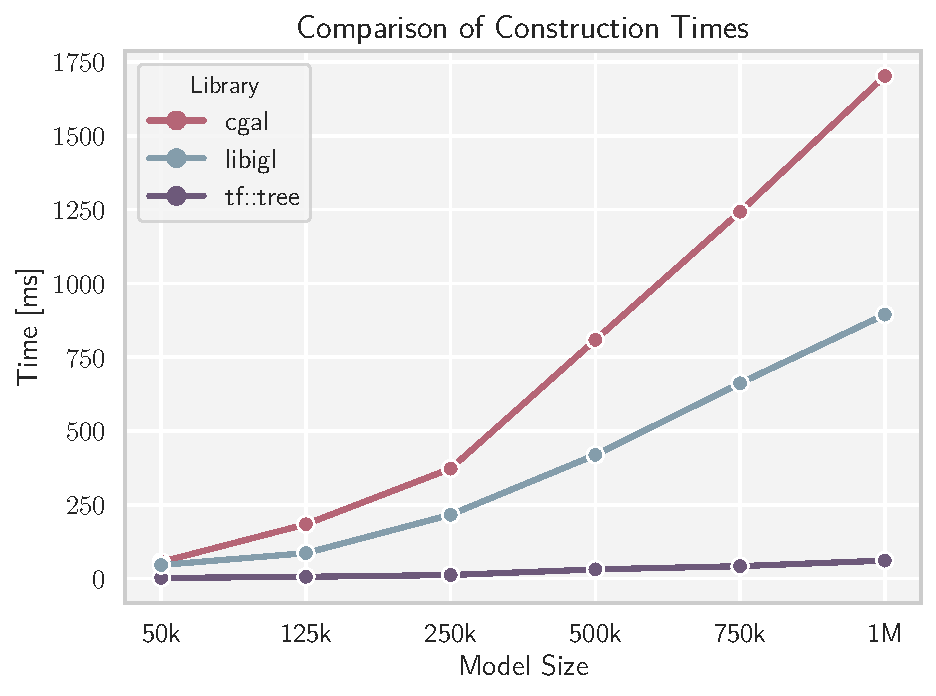
\includegraphics[width=\linewidth]{../figures/libraries-cons.pdf}
\caption{
Tree construction times for models from 50k to 1M triangles using \texttt{tf::tree}, CGAL, and libigl.
\texttt{tf::tree} is significantly faster, building a 1M-triangle model in 52\,ms versus 894\,ms (libigl) and 1.7\,s (CGAL),
highlighting its suitability for real-time applications.
}
\label{fig:lib-comparison}
\end{figure}


Open-source libraries offering spatial acceleration structures can be
broadly divided into three categories: those optimized for ray tracing,
those optimized for collision detection and physics,
and those designed for general-purpose geometric processing.
\texttt{tf::tree} belongs to the third category.

Libraries such as Embree~\cite{embree}, OptiX~\cite{optix}, and nanort\cite{nanort}
are highly optimized for ray tracing and real-time rendering workloads.
These systems emphasize ray traversal speed and often rely on SAH-based
hierarchies tailored for directional queries. However, their APIs and
internal designs make them less suitable for general spatial queries such
as collision detection, primitive intersection, or proximity-based reasoning.

A second category, including libraries for real-time physics and robotics
like Bullet Physics~\cite{bullet} and FCL~\cite{fcl}, prioritizes fast and
stable collision detection for simulations. Their algorithms are often tuned
with concepts like collision margins, making them unsuitable for fine-grained
geometric modeling tasks, such as collecting the complete set of primitive
intersections required for mesh booleans.

Finally, libraries like CGAL~\cite{cgal} and libigl~\cite{libigl}
provide general-purpose tools for geometric computation. While
these libraries support a wide range of operations, including
boolean modeling and proximity tests, their acceleration structures
are often not optimized for real-time performance. They may also lack
the fine-grained control over traversal, construction strategies,
and query types that \texttt{tf::tree} offers. A comparison of
construction times is presented in Figure~\ref{fig:lib-comparison}.
